\documentclass{article}
\usepackage[utf8]{inputenc}
\usepackage{array}
\usepackage{wrapfig}
\usepackage{multirow}
\usepackage{tabu}
\usepackage{graphics}
\usepackage{graphicx}

\title{Report}
\author{Yusif Aliyev}
\date{18.05.2021}

\begin{document}

\maketitle
\section{Part 1: K-Nearest Neighbor}
\subsection{K-fold Cross-validation}
The below graph represents k-fold cross validation with the average accuracy values on the $y$ axis and $k$ values on the $x$ axis
with k=1,2,3,...,199. Red dot represents maximum accuracy value.
\begin{figure}[htp]
    \centering
    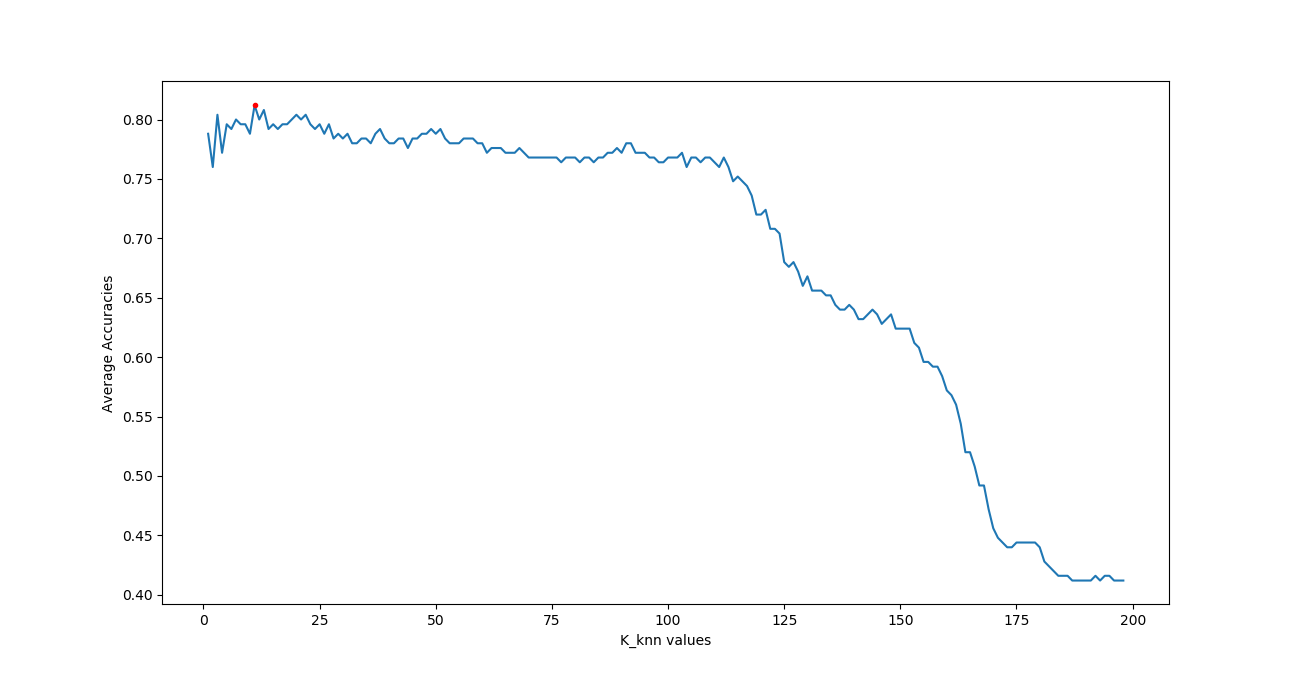
\includegraphics[width=16cm]{Figure_1_marked.png}
    \caption{K-fold cross validation graph}
    \label{fig:fig1}
\end{figure}

\subsection{Accuracy drops with very large k values}
While increasing the $k$ value to the very large point, overfitting will be happened, because with such high value of $k$, it can 
cover most of the data points, such that decision boundary becomes smoother and more resilient to outliers and thus resulting in reduced variance and high bias.

\subsection{Accuracy on test set with the best k}
Maximum average validation accuracy is $0.79$.The best test set accuracy value is $0.82$ with the best value of $k_{KNN}=11$.


\maketitle
\section{Part 2: K-means Clustering}
\subsection{Elbow method}
\begin{figure2}
    \centering
    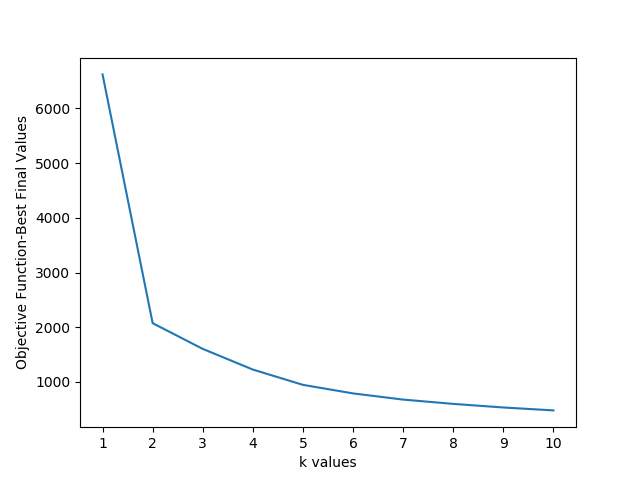
\includegraphics[width=14cm]{Elbow-cluster1.png}
    \caption{Figure 2: Elbow method graph for Clustering 1 (suitable $k=2$)}
    \label{fig:fig2}
\end{figure2}

\begin{figure3}
    \centering
    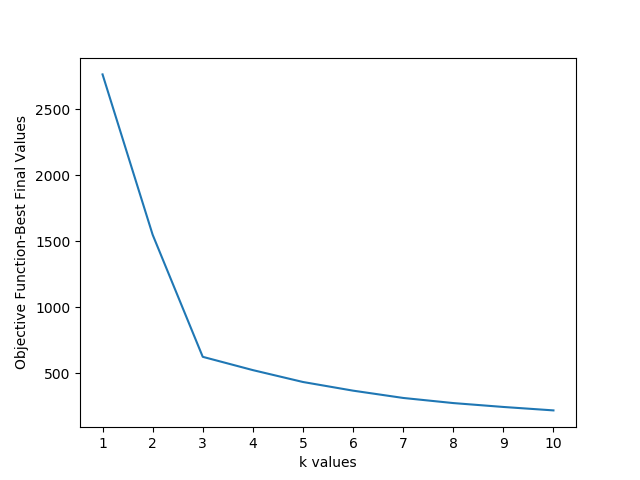
\includegraphics[width=14cm]{Elbow-cluster2.png}
    \caption{Figure 3: Elbow method graph for Clustering 2 (suitable $k=3$)}
    \label{fig:fig3}
\end{figure3}

\begin{figure4}
    \centering
    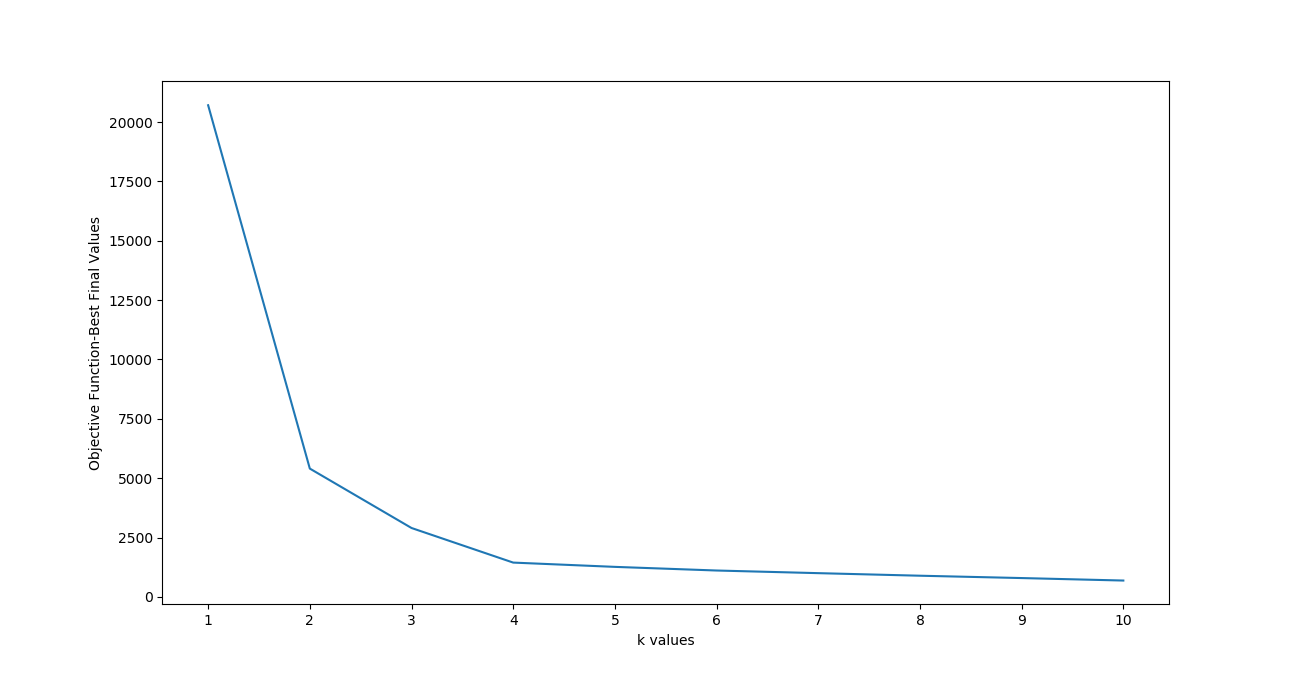
\includegraphics[width=14cm]{Elbow-cluster3.png}
    \caption{Figure 4: Elbow method graph for Clustering 3 (suitable $k=4$)}
    \label{fig:fig4}
\end{figure4}

\begin{figure5}
    \centering
    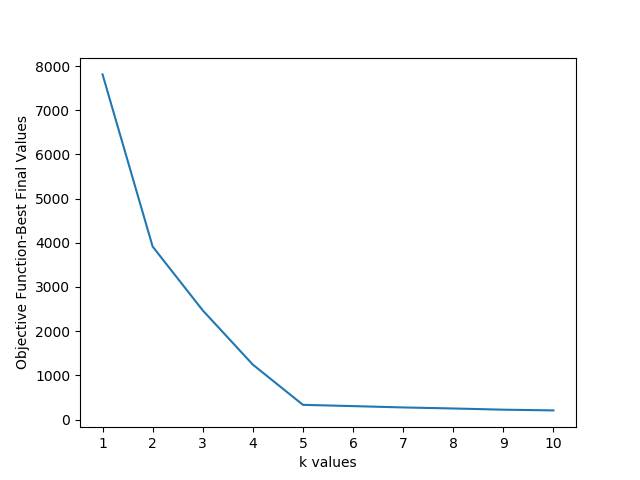
\includegraphics[width=14cm]{Elbow-cluster4.png}
    \caption{Figure 5: Elbow method graph for Clustering 4 (suitable $k=5$)}
    \label{fig:fig5}
\end{figure5}
\subsection{Resultant Clusters}
There are resultant clusters plots for each clustering data below:

\begin{figure6}
    \centering
    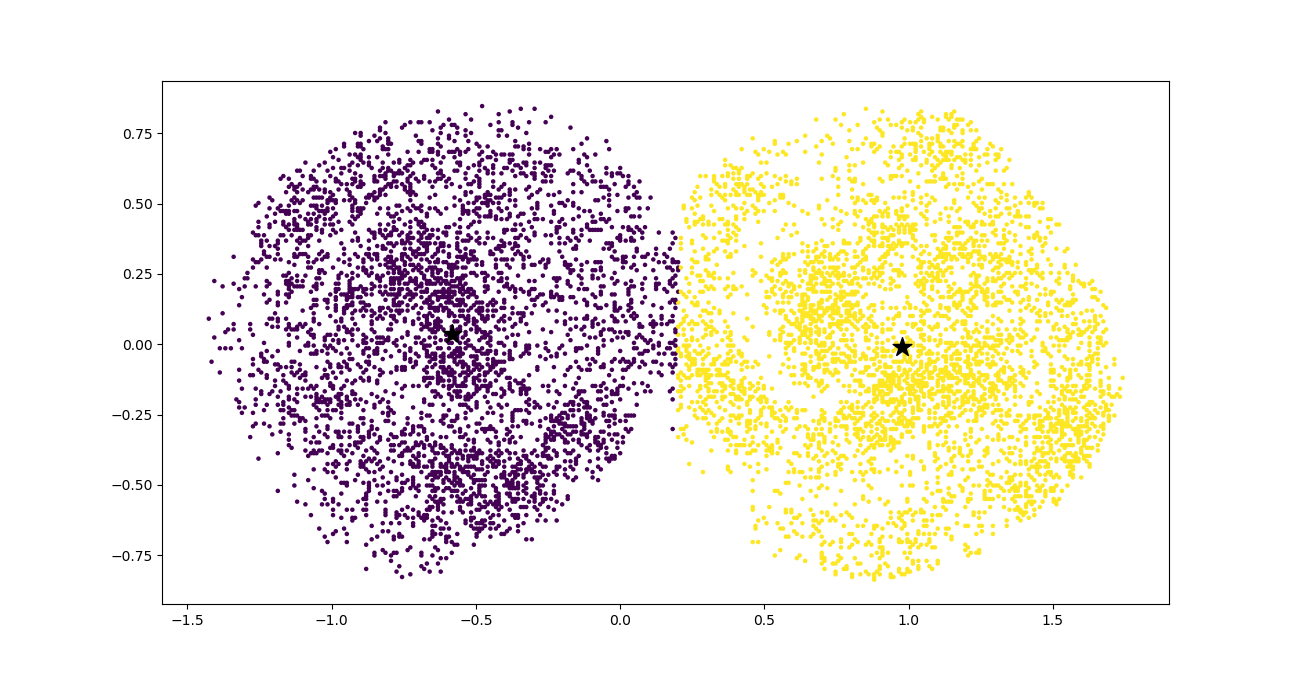
\includegraphics[width=14cm]{cluster1.png}
    \caption{Figure 6: Resultant Cluster 1 (with the value of $k=2$)}
    \label{fig:fig6}
\end{figure6}

\begin{figure7}
    \centering
    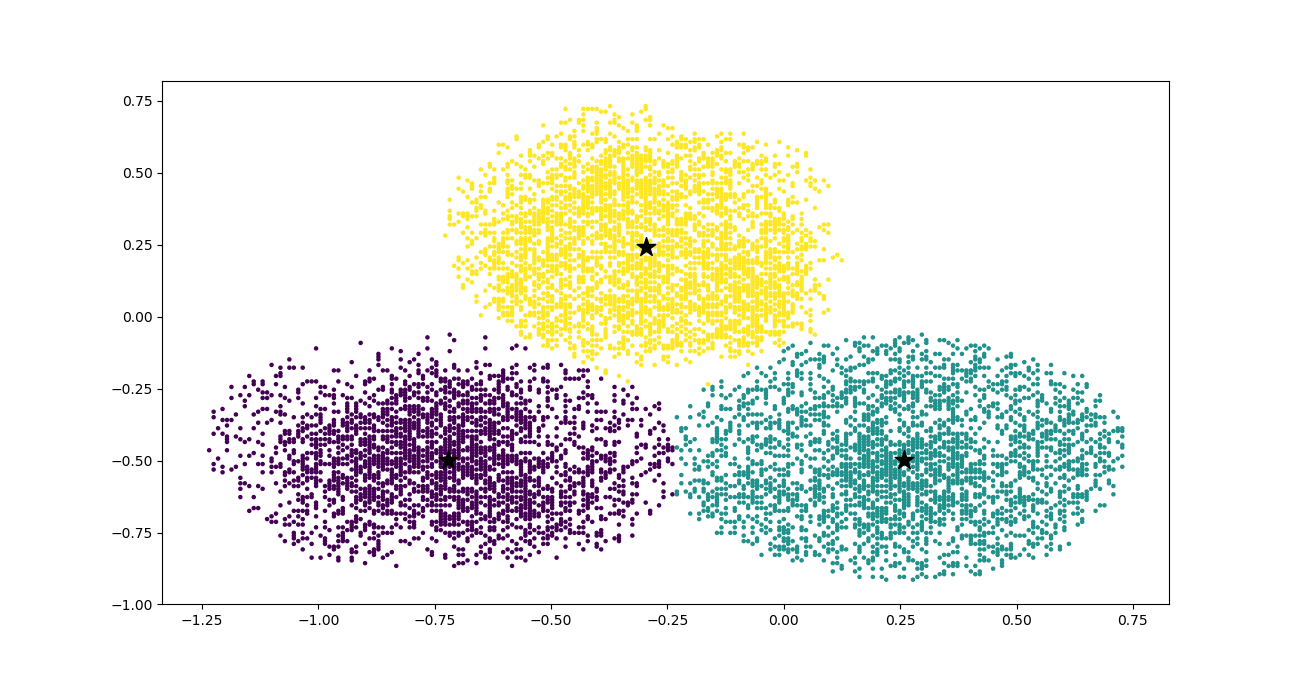
\includegraphics[width=14cm]{cluster2.png}
    \caption{Figure 7: Resultant Cluster 2 (with the value of $k=3$)}
    \label{fig:fig7}
\end{figure7}

\begin{figure8}
    \centering
    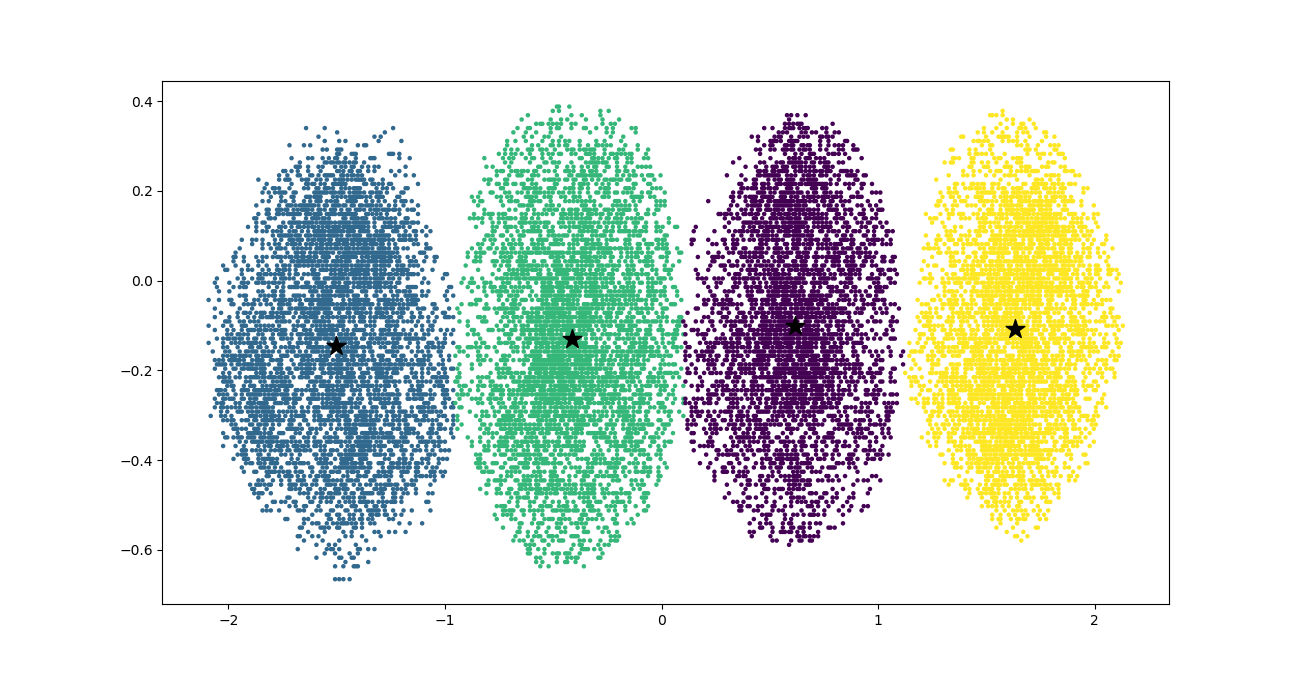
\includegraphics[width=14cm]{cluster3.png}
    \caption{Figure 8: Resultant Cluster 3 (with the value of $k=4$)}
    \label{fig:fig8}
\end{figure8}

\begin{figure9}
    \centering
    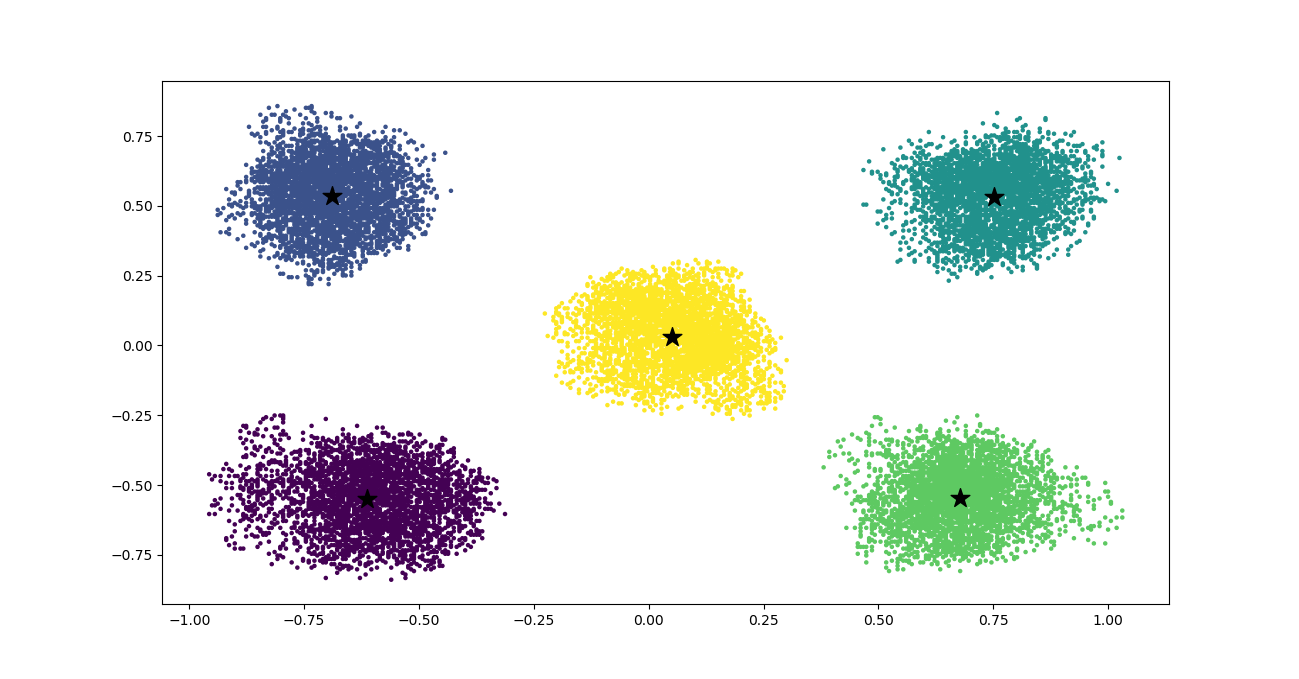
\includegraphics[width=14cm]{cluster4.png}
    \caption{Figure 9: Resultant Cluster 4 (with the value of $k=5$)}
    \label{fig:fig9}
\end{figure9}

\maketitle
\section{Part 3: Hierarchical Agglomerative Clustering}
\subsection{data1}
Plot the resultant clusters using each criterion and \textbf{shortly comment on their behaviour and why they work in that way}.\\
\subsection{data2}
Plot the resultant clusters using each criterion and \textbf{shortly comment on their behaviour and why they work in that way}.\\
\subsection{data3}
Plot the resultant clusters using each criterion and \textbf{shortly comment on their behaviour and why they work in that way}.\\
\subsection{data4}
Plot the resultant clusters using each criterion and \textbf{shortly comment on their behaviour and why they work in that way}.\\

\end{document}

